\documentclass[a4paper,openright, 12pt]{book}
\usepackage[spanish]{babel} 
\usepackage[utf8]{inputenc} 
\usepackage{listings}
\usepackage{color}
\usepackage{amsmath}
\usepackage{mathtools}
\usepackage{graphicx}
\usepackage{url}

\definecolor{mygreen}{rgb}{0,0.6,0}
\definecolor{mygray}{rgb}{0.5,0.5,0.5}
\definecolor{mymauve}{rgb}{0.58,0,0.82}


\spanishdecimal{.}

\lstset{ %
  backgroundcolor=\color{white},   
  basicstyle=\ttfamily,       
  breakatwhitespace=false,         
  breaklines=true,                 % sets automatic line breaking
  captionpos=b,                    % sets the caption-position to bottom
  commentstyle=\color{mygreen},    % comment style
  columns=flexible,
  deletekeywords={...},            % if you want to delete keywords from the given language
  escapeinside={\%*}{*)},          % if you want to add LaTeX within your code
  extendedchars=true,              % lets you use non-ASCII characters; for 8-bits encodings only, does not work with UTF-8
  frame=single,                    % adds a frame around the code
  keepspaces=true,                 % keeps spaces in text, useful for keeping indentation of code (possibly needs columns=flexible)
  keywordstyle=\color{blue},       % keyword style
  language=Python,                 % the language of the code
  morekeywords={*,...},            % if you want to add more keywords to the set
  numbers=left,                    % where to put the line-numbers; possible values are (none, left, right)
  numbersep=5pt,                   % how far the line-numbers are from the code
  numberstyle=\tiny\color{mygray}, % the style that is used for the line-numbers
  rulecolor=\color{black},         % if not set, the frame-color may be changed on line-breaks within not-black text (e.g. comments (green here))
  showspaces=false,                % show spaces everywhere adding particular underscores; it overrides 'showstringspaces'
  showstringspaces=false,          % underline spaces within strings only
  showtabs=false,                  % show tabs within strings adding particular underscores
  stepnumber=1,                    % the step between two line-numbers. If it's 1, each line will be numbered
  stringstyle=\color{mymauve},     % string literal style
  tabsize=4,                       % sets default tabsize to 2 spaces
  title=\lstname                   % show the filename of files included with \lstinputlisting; also try caption instead of title
}




\begin{document}

\begin{titlepage}
\begin{center}
\begin{Huge}
\textsc{Título}
\end{Huge}
\end{center}
\end{titlepage}

\newpage
\mbox{}
\thispagestyle{empty} 


\tableofcontents % indice de contenidos
\newpage
\thispagestyle{empty}


\chapter*{Motivación}\label{cap.introduccion}
\addcontentsline{toc}{chapter}{\protect\numberline{}Motivación}%
\pagenumbering{arabic} % para empezar la numeración con números

El interés inicial y motivo principal para la realización de este trabajo fue el acercamiento al interesante mundo de la visión artificial. Los campos relacionados con la visión artificial son amplísimos, abarcando casi la totalidad de las actuales actividades que incorporan algún tipo de imagen a su tecnología . El verdadero problema inicial fue elegir en qué centrar el interés de las numerosísimas actividades y tareas relacionadas con la visión artificial. Por acotar un poco el terreno, mi interés dentro de la visión artificial estaba en algo que tuviese una aplicación real en el mundo. Acudí a la presentación de una aplicación para móviles llamada Mememtum \footnote{\url{http://mememtum.com}}. Esta aplicación, que se encuentra aún en una primera versión, pretende proporcionar una manera de controlar la evolución del Parkinson y otros trastornos del movimiento a los pacientes desde su casa a través del móvil. Por supuesto, esta aplicación usa visión artificial; por ello, hablé con uno de los responsables del proyecto. Me dijo que algunos de los problemas que tenían en esta versión estaban relacionados con la estabilización de la imagen y la iluminación y, por ello, me sugirió que podía orientar mi trabajo en esta dirección.


Esta aplicación para el control del Parkinson consiste en que una segunda persona graba al enfermo de Parkinson y tras procesar el vídeo, devuelve un número que representa la cantidad de movimiento del paciente y que se puede utilizar para hacer un seguimiento del mismo. Podría considerarse como un ``termómetro del Parkinson''. El problema que surge con una aplicación para el móvil es que al movimiento del enfermo, hay que sumarle el posible movimiento involuntario de la cámara producido por la persona que está grabando. El reto, por tanto, está en intentar eliminar dicho movimiento involuntario. Una idea que me sugirieron era, ya que estaban trabajando con móviles, intentar aprovechar los sensores de que estos disponen, como el acelerómetro, para corregir este  movimiento.
\newpage
Finalmente decidí realizar el trabajo en esta dirección, y por tanto centrarme en las tareas de: estabilización de la imagen con algoritmos de visión artificial, intentar estabilizar la imagen con ayuda de los datos del aceleŕometro y estabilización de la iluminación.
En primer lugar, para poder realizar los algoritmos de visión artificial tuve que aprender a utilizar la librería openCV y familiarizarme con algunos algoritmos típicos de visión artificial. Además como iba a intentar hacer uso del acelerómetro, tuve que aprender a realizar aplicaciones para Android y cómo interactuar con el hardware de los móviles. Tras todo este trabajo previo ya estaba en condiciones de centrarme en las tareas anteriormente mencionadas.

Por tanto, el trabajo está estructurado de la siguiente manera:
en primer lugar un capítulo dando una breve visión de conjunto de OpenCV y algunos códigos sencillos de ejemplo que hice durante el proceso de aprendizaje.
\newline
El siguiente capítulo está dedicado a otras librerías que, sin jugar un papel tan protagonista como OpenCV, he tenido que aprender y usar durante el trabajo. La parte central de este capítulo es Android y una pequeña noción de cómo se estructuran este sistema operativo y sus aplicaciones.
\newline
El siguiente capítulo trata sobre la estabilización de la imagen y abarca tanto los algoritmos puramente de visión artificial para estabilizar la imagen, como los intentos de usar el acelerómetro con este objeto. Cabe señalar que, debido a las motivaciones del trabajo comentadas anteriormente, durante todo el capítulo se supondrá que la cámara está estática, en el sentido de que el único movimiento producido por esta es leve y es el que queremos corregir.
\newline
Y finalmente el último capítulo está dedicado a la estabilización de la luz.

\chapter{OpenCV}

\section{Introducción}
OpenCV es una librería de código abierto escrita en C y C++ destinada a la visión artificial y al tratamiento de imágenes. Se trata de una librería multiplataforma con versiones para GNU/Linux, Windows, Mac OS y Android y actualmente cuenta con interfaces para Python, Java y MATLAB/OCTAVE. Las últimas versiones incluyen soporte para CUDA, lo que nos permite ejecutar paralelamente funciones en la unidad de procesamiento gráfico o GPU de nuestro ordenador .
Desarrollada originalmente por Intel, su primera versión alfa se publicó en el año 2000 en el \textit{IEEE Conference on Computer Vision and Pattern Recognition}. OpenCV nació inicialmente como un proyecto para avanzar en las aplicaciones de uso intenso de la CPU y dando gran importancia a las aplicaciones en tiempo real. Hoy en día cuenta con más 2500 algoritmos optimizados que abarcan todo tipo de campos relacionados con la visión artificial.
Estos algoritmos pueden ser usados para tareas como: detección y reconocimiento de caras y gestos, identificación objetos, detección de características 2D y 3D, estimación y seguimiento del movimiento, visión estéreo y calibración de la cámara, eliminación los ojos rojos de las fotografías realizadas con flash...
\newline
OpenCV es ampliamente utilizada por todo tipo de empresas (desde grandes empresas como Google, Yahoo, Microsoft, Intel, IBM, Sony, Honda, Toyota a pequeñas empresas), grupos de investigación y organismos gubernamentales y en sectores de todo tipo como: inspección de los productos en las fábricas, seguridad, usos médicos, robótica...
\newline
Como ya hemos dicho, openCV incluye todo tipo de funciones e implementaciones de algoritmos. 
Dichas funciones se pueden dividir en varios grupos:
\begin{itemize}
\item Las relacionadas con el interfaz gráfico: se encargan de crear ventanas, mostrar imágenes por pantalla, registrar las pulsaciones del teclado, y de crear la interfaz de usuario (botones, barras de desplazamiento, etc). Veremos las más importantes en los ejemplos de la sección siguiente.
\item Las estructuras básicas como las matrices y las funciones para trabajar con ellas. En la versión para python esto no es muy importante porque está adaptada para trabajar con arrays de Numpy (una extensión para python que añade funciones para el cálculo científico y sobre la que hablaremos un poco más en detalle en el siguiente capítulo).
\item Las funciones de procesado de imágenes. Es la parte fundamental de openCV y contiene funciones de todo tipo: 
\begin{itemize}
\item Filtros de imagen, como desenfoques varios, ampliar o reducir una imagen, calcular el gradiente de una imagen mediante el operador Sobel...
\newline Veremos algunas de estas funciones en los ejemplos.
\item Transformaciones geométricas. Estas funciones realizan diversas tareas de carácter geométrico sobre las imágenes 2D, como calcular la transformación afín que lleva unos puntos a otros, calcular la matriz de una rotación o aplicarle a una imagen la matriz de una transformación.
\item Funciones relacionadas con el cálculo y manejo de histogramas (comparar dos histogramas, normalizar un histograma...).
\item Funciones de estimación de movimiento y detección de características. La más importantes son usadas y explicadas en el capítulo 4.
\end{itemize}
\item Funciones de calibrado de la cámara (para corregir la distorsión provocada por la lente) y de reconstrucción 3D usando visión estéreo (dos cámaras).
\item Funciones para detectar objetos y caras. Destaca la clase \lstinline|CascadeClassifier|.
\item Además, openCV consta de una librería de aprendizaje automático (\textit{machine learning}) que está formada por funciones de clasificación estadística, árboles de decisión, redes neuronales...
\end{itemize}
Por supuesto openCV es una librería enorme y consta de muchísimas más funciones que las aquí mencionadas\newpage
\section{Ejemplos}
A continuación veremos una serie de ejemplos sencillos de uso de openCV con Python, similares a los propuestos en el capítulo 2 de \textit{"Learning OpenCV" \cite{oreilly}}. No obstante en el libro estos ejemplos están programados en C con una versión antigua de la librería y aquí se presentan en Python y actualizados. Al tratarse de una librería tan extensa, es imposible cubrirla o resumirla en unos ejemplos. Por tanto, los códigos que vienen a continuación pretenden tan solo dar una idea de algunos funciones básicas a hora de trabajar con la librería como abrir y mostrar vídeos e imágenes y algunas transformaciones sencillas.
\subsection*{Ejemplo 1}
En primer lugar veamos como mostrar una imagen en una ventana
\lstinputlisting[language=Python, frame= single]{ejemplos/ejemplo1.py}
Como vemos se trata de un código muy sencillo. Al ser ejecutado con un argumento, carga una imagen y la muestra en una ventana; luego espera hasta que el usuario pulse una tecla.

La función \lstinline|cv2.imread()| es la que se encarga de cargar la imagen desde un archivo.  Esta función toma como argumentos el nombre del archivo que se quiere abrir y además podemos especificar con un segundo parámetro opcional el modo de color en que se carga la imagen.

La función devuelve la imagen (en forma de array de Numpy).
\newline
Una vez hemos cargado la imagen, la mostramos en una ventana usando \lstinline|cv2.imshow(winname, image)|, donde \lstinline|winname| es el nombre de la ventana e \lstinline|image| es la imagen que queremos mostrar.
Por último, utilizamos \lstinline|cv2.waitKey(0)| para esperar a que el usuario pulse una tecla. Esta función recibe un único parámetro que indica el tiempo de espera en milisegundos para la pulsación de una tecla. Si este parámetro es menor o igual que cero, esperará indefinidamente.

\subsection*{Ejemplo 2}
En el siguiente ejemplo vemos como cargar un archivo de vídeo y mostrarlo en una ventana. El programa termina cuando el vídeo se acaba o cuando el usuario pulsa la tecla ``Esc"
\lstinputlisting[language=Python, frame= single]{ejemplos/ejemplo2.py}
En este ejemplo hemos hecho uso de la clase VideoCapture.
La función \lstinline|cv2.VideoCapture(filename)| recibe como argumento el nombre de un archivo de video o la ID de un dispositivo de video (en este caso un nombre de archivo) y devuelve un objeto de la clase VideoCapture.
De esta clase tan solo usamos ahora la función \lstinline|cv2.VideoCapture.read()| que toma el siguiente fotograma, lo decodifica y lo devuelve. Además de la imagen, devuelve un booleano, que en el código hemos llamado ``\lstinline|ret|", que es \textit{\lstinline|False|} si ningún fotograma ha sido tomado y \textit{\lstinline|True|} en otro caso.
Como ahora ya tenemos una imagen, para mostrarla por pantalla usamos la misma función que en el ejemplo 1.
Por último, esta vez usamos la función \lstinline|cv2.waitKey| de manera un poco distinta al anterior ejemplo. Como ahora estamos en un bucle, esperamos a la pulsación 33 milisegundos. Si alguna tecla es pulsada, su valor ASCII se almacena y lo comparamos con 27 que es el correspondiente a la tecla ``Esc".

\newpage
\subsection*{Ejemplo 3}
En este ejemplo mejoraremos un poco el reproductor de vídeo que hemos programado en el ejemplo anterior. Se ha añadido una barra de deslizamiento con el instante del vídeo en que nos encontramos, el cual se puede utilizar para avanzar y retroceder hasta donde deseemos.
\lstinputlisting[language=Python, frame= single, firstline=4, lastline=27]{ejemplos/ejemplo3.py}
Como vemos, en este código hemos introducido unas cuantas funciones nuevas.
En primer lugar, hemos usado varias veces la función \lstinline|cv2.VideoCapture.get(propId)| con distintos argumentos.
Esta función devuelve el valor de distintas propiedades del video con el que estamos trabajando. El argumento es el identificador de la propiedad entre los que destacan: \lstinline|CV_CAP_PROP_POS_FRAMES| (posición del próximo fotograma que va a ser decodificado/capturado), \lstinline|CV_CAP_PROP_FPS| (fotogramas por segundo) y \lstinline|CV_CAP_PROP_FRAME_WIDTH|y \lstinline|CV_CAP_PROP_FRAME_HEIGHT| (anchura y altura de los fotogramas del video respectivamente).
La lista completa de opciones puede ser encontrada fácilmente en la documentacíon de openCV.

También usamos la función \lstinline|cv2.VideoCapture.set(propId, value)|, usada para fijar el valor de alguna de las propiedades del vídeo. Por tanto los valores que puede tomar \lstinline|propId| son los mismos que para la función \lstinline|cv2.VideoCapture.get()| y el argumento \lstinline|value| indica el nuevo valor que tomará la propiedad indicada.

Una vez cargamos el video como ya sabemos y obtenemos el número total de fotogramas con la función \lstinline|get| como acabamos de ver, procedemos a crear una ventana con la función \lstinline|cv2.namedWindow(winname[, flags])|.
Hasta ahora no había hecho falta ya que \lstinline|cv2.imshow| creaba una nueva ventana si no existía una con ese nombre.
Ahora le vamos a añadir algo (una trackbar) a nuestra ventana, por lo que necesitamos que ya esté creada.
Para esto usamos \lstinline|cv2.createTrackbar(trackbarName, windowName, value, count, onChange)|, siendo estos parámetros el nombre de la barra de deslizamiento creada, el nombre de la ventana en la que queremos la barra,una variable que refleja la posición del deslizador, la posición máxima del deslizador (la posición mínima es 0 siempre) y por último una función que será llamada cada vez que la barra de deslizamiento cambie de posición.

\newpage

\subsection*{Ejemplo 4}
Ahora vamos a ver un ejemplo de una transformación muy sencilla, vamos a abrir una imagen y a aplicarle un desenfoque gaussiano y a mostrar tanto la imagen original como la resultante por pantalla. El desenfoque gaussiano es un filtro usado para suavizar imágenes y desenfocarlas. Funciona de la siguiente manera: cada píxel de la imagen mezcla su color con los de un ventana a su alrededor (de altura y anchura dadas). Esta mezcla es una media de los píxeles que están dentro de la ventana ponderada con un núcleo gaussiano (es decir la media de los píxeles multiplicando cada uno de ellos por un peso, que en este caso lo da el núcleo gaussiano\footnote{Un núcleo gaussiano de tamaño $\texttt{ksize}$ es una matriz de dimensiones $ \texttt{ksize}\times1$ con coeficientes:
$ G_i= \alpha *e^{-(i-( \texttt{ksize} -1)/2)^2/(2* \texttt{sigma} )^2}$ donde i va de $0$ a$\texttt{ksize}-1$ y $\alpha$ es tal que  $\sum_i G_i=1$. }). 
\lstinputlisting[language=Python, frame= single]{ejemplos/ejemplo4.py}
La única función nueva es 
\lstinline|cv2.GaussianBlur()|, que es la que realiza el desenfoque.
Sus parámetros obligatorios son la imagen y el tamaño del núcleo. Puede además indicarse los valores $\sigma_1$ y $\sigma_2$. Si ambos son 0, entonces se calcularán a partir del tamaño del núcleo $(k_1, k_2)$ con la siguiente fórmula:
\begin{equation*}
\sigma_1 = 0.3\cdot(\frac{k_1-1}{2} - 1) + 0.8
\end{equation*}
\begin{equation*}
\sigma_2 = 0.3\cdot(\frac{k_2-1}{2} - 1) + 0.8
\end{equation*}



\newpage

\subsection*{Ejemplo 5}
En este ejemplo realizamos otra transformación, en este caso reducimos la imagen a la mitad. Esta tarea la realiza la función \lstinline|cv2.pyrDown|
\lstinputlisting[language=Python, frame= single]{ejemplos/ejemplo5.py}
Como vemos, en el resto del código no hay nada nuevo, a excepción de la función ya nombrada.
\newpage
\subsection*{Ejemplo 6}
En este ejemplo utilizamos el algoritmo de Canny \cite{canny86} de detección de bordes, usando para ello la función \lstinline|cv2.Canny|.
 Este algoritmo funciona de la siguiente manera: en primer lugar aplica un desenfoque gaussiano a la imagen para reducir el ruido. Posteriormente calcula el gradiente de la imagen. Esto lo hace aplicando dos matrices de convolución para calcular las derivadas en las direcciones $x$ e $y$:

\begin{equation*}
G_{x} = \begin{bmatrix} -1 & 0 & +1 \\ -2 & 0 & +2 \\ -1 & 0 & +1 \end{bmatrix},  G_{y} = \begin{bmatrix} -1 & -2 & -1 \\ 0 & 0 & 0 \\ +1 & +2 & +1 \end{bmatrix}
\end{equation*}

Para finalmente calcular el gradiente y su dirección:

\begin{equation*}
\begin{array}{l} G = \sqrt{ G_{x}^{2} + G_{y}^{2} } \\ \theta = \arctan(\dfrac{ G_{y} }{ G_{x} }) \end{array}
\end{equation*}
Por último, para decidir si los píxeles pertenecen a un borde, se utilizan dos umbrales, uno superior y otro inferior:
\begin{itemize}
\item Si el gradiente del píxel es mayor que el umbral superior, se acepta el píxel como borde.
\item Si el gradiente del píxel es menor que el umbral inferior, se rechaza el píxel.
\item Si el gradiente está entre ambos umbrales, entonces se acepta solo si está conectado a un píxel que está por encima del umbral superior.
\end{itemize}

A continuación vemos un ejemplo que muestra la imagen de la \textit{webcam} y utiliza el algoritmo de Canny de detección de bordes.

\newpage
\lstinputlisting[language=Python, frame= single]{ejemplos/ejemplo6.py}
Como vemos el código para mostrar una imagen de la \textit{webcam} es exactamente el mismo que el de mostrar un vídeo por pantalla, excepto que a la función \lstinline|cv2.VideoCapture| le pasamos como argumento, en lugar del nombre del archivo, un entero que representa el índice de la cámara (si solo hay una cámara, debe ser 0).
\newpage

\newpage 
\subsection*{Ejemplo 7}
Ahora simplemente vamos a combinar los dos ejemplos anteriores, reduciendo dos veces la imagen original con \lstinline|pyrDown| y luego encontrando los bordes con \lstinline|Canny|
\lstinputlisting[language=Python, frame= single]{ejemplos/ejemplo7.py}
\newpage

\chapter{Otras librerías usadas}
\section{Android}

Android es un sistema operativo desarrollado por Google y orientado a móviles y tablets. Está basado en Linux y es de código abierto. Actualmente se estima que en torno a un 80\% de los dispositívos móviles usan el sistema operativo Android.
Su núcleo está programado en C, pero la aplicaciones y toda la interfaz de usuario se programan en Java.
Este sistema operativo está estructurado en 4 capas:
\begin{description}
  \item[Núcleo Linux] \hfill \\
  Se encarga de las funcionalidades básicas del sistema, como manejo de procesos, de la memoria y de los dispositivos como la cámara, la pantalla, etc.
   Asimismo funciona como una capa de abstracción entre el \textit{hardware} y el resto del \textit{software}.
   
  \item[Librerías y \textit{runtime} de Android] \hfill \\
  Por encima del núcleo, hay una serie de librerías usadas por componentes del sistema, entre ellas destacan Surface Manager, Media Framework, SQLite, WebKit, SGL y Open GL
  \newline
  El runtime de Android proporciona un componente clave,la máquina virtual Dalvik. Cada aplicación Android corre su propio proceso, con su propia instancia de esta máquina virtual.
  Además, el \textit{runtime} de Android proporciona librerías básicas que proporcionan la mayor parte de las funciones del lenguaje de programación Java.
  
  \item[Marco de trabajo(\textit{framework}) de aplicaciones] \hfill \\
  Esta capa proporciona a las aplicaciones muchos servicios en forma de clases de Java 
  
   \item[Aplicaciones] \hfill \\
  En esta capa se encuentran tanto las aplicaciones base como las que instalemos y desarrollemos. Como ya hemos dicho estas aplicaciones se programan en Java, disponiendo para ello del conjunto de herramientas Android SDK.
\end{description}

\subsection*{Estructura de una aplicación Android}
Las aplicaciones Android están formadas por los llamados componentes de aplicación. Hay cuatro tipo de componentes:
\begin{description}
  \item[Activities] \hfill \\
  Representa una única pantalla de la aplicación con su interfaz de usuario.
  \item[Services] \hfill \\
  Son componentes que se ejecutan en segundo plano y que no constan de interfaz gráfica.
  \item[Content providers] \hfill \\
  Se encarga de compartir información entre distintas aplicaciones.
  \item[Broadcast receivers] \hfill \\
  Este componente permite el registro de eventos del sistema
\end{description}
La aplicaciones que nosotros vamos a realizar son muy sencillas y solo utilizarán el primero de todos estos componentes.
Una vez visto esto veamos por encima la estructura de una aplicación Android.
Dichas aplicaciones vienen en formato APK, que no es más que un fichero comprimido ZIP en el que se encuentran: el código, los recursos, la firma digital y el fichero de manifiesto.
\newline
Los recursos se encuentran en la carpeta \lstinline|res|. Además de las imágenes y otro tipo de contenido que usemos en la aplicación, esta carpeta contiene otra carpeta, llamada \lstinline|layouts|, en la que se encuentran archivos XML que describen las distintas pantallas o vistas de cada aplicación, es decir las interfaces gráficas asociadas a cada actividad.
\newline
El archivo ``\lstinline|manifest.xml|'' es un fichero XML donde se declaran los componentes que conforman la aplicación, así como se indican los permisos necesarios que requiere la aplicación, las funciones de \textit{hardware} o \textit{software} que se necesitan (la cámara, el acelerómetro, los servicios de \textit{bluetooth}...) y algunas características más del programa.

En el apéndice \ref{android_ap_acc} se incluye el código de Android realizado, donde se pueden ver el código de la actividad principal y su \lstinline|layout|, así como el fichero ``\lstinline|manifest.xml|''.

\section{Numpy}
Numpy (NUMerical PYthon) es una extensión para Python que agrega una gran cantidad de funcionalidades para el calculo matemático. La más destacable que incorpora es el soporte para arrays n-dimensonales y funciones para operar con ellos. Además incluye numerosas funciones de álgebra lineal, transformadas de Fourier, estadística básica...
\newline
El núcleo de Numpy es el objeto \lstinline|ndarray|, que es la estructura de datos que representa los arrays n-dimensionales. Estos arrays, a diferencia de las listas de Python, deben estar formados por elementos del mismo tipo.
La manera más usual de crear estos arrays es a partir de una lista de Python: \lstinline|numpy.array([1,2,3,4])|. También pueden usarse las funciones \lstinline|numpy.zeros(n,m)| y \lstinline|numpy.ones((n,m))| para crear matrices $nxm$ formadas solo por ceros o por unos, respectivamente.
\newline
Los operadores aritméticos pueden usarse con los arrays y se aplican elemento a elemento y devuelven un nuevo array con el resultado.
El operador \lstinline|*| es la multiplicación elemento a elemento, para la multiplicación de matrices se usa la función \lstinline|numpy.dot(A,B)|.
Otros ejemplos de funciones son: \lstinline|numpy.sum()|,\lstinline|numpy.min()| y \lstinline|numpy.max()|.

Los principales atributos de \lstinline|ndarray| son:
 \begin{itemize}
\item \lstinline|ndarray.ndim|: el número de dimensiones (o ejes) del array.
 
\item \lstinline|ndarray.shape|: las dimensiones del array. Consiste en una tupla (de longitud \lstinline|ndim|) de enteros que indican el tamaño del array en cada dimensión. Por ejemplo, para una matriz de $n$ filas y $m$ columnas, será (n,m).

\item  \lstinline|ndarray.size|: el número total de elementos del array. Es el producto de todos los elementos de \lstinline|shape|. 

\item\lstinline|ndarray.dtype|: el tipo de los elementos del array. Se pueden crear o especificar tipos usando los tipos estándar de Python. Además Numpy proporciona algunos tipos más, como \lstinline|numpy.int32|, \lstinline|numpy.int16|, y \lstinline|numpy.float64|

\item \lstinline|ndarray.data|: el búfer que contiene los elementos del array. Generalmente no se usa este atributo ya que se suele acceder a los elementos usando índices.
 \end{itemize}
Nuestras imágenes de OpenCV serán arrays de Numpy cuyo atributo \lstinline|ndim| será 2 si la imagen es en blanco y negro y 3 si tiene más de un canal.
El atributo \lstinline|shape| será de la forma \lstinline|(h,w,n)| (o \lstinline|(h,w)| si es en blanco y negro), donde \lstinline|h| es la altura de la imagen, \lstinline|w| es el ancho y \lstinline|n| es el número de canales de la imagen.
\chapter{Estabilización de imagen}\label{cap.}

\section{Algoritmo básico}
Se trata de un algoritmo básico de estabilización de imagen para eliminar el posible movimiento de agitación la cámara. Dicho algoritmo se basa en la suposición de que el único movimiento de la cámara es el que queremos eliminar; es decir, excepto por ligeros movimientos no deseados, la cámara está estática.
La idea del algoritmo es muy sencilla: 
Tomamos dos fotogramas consecutivos y buscamos una serie de puntos característicos mediante el algoritmo propuesto por Shi y Tomashi \cite{shiandtomasi}, usando la función: \lstinline|goodFeaturesToTrack|; después vemos a donde se han movido esos puntos en el siguiente fotograma mediante el algoritmo de flujo óptico de Lucas-Kanade.
Finalmente calculamos la homografía que lleva los puntos originales a donde hemos calculado que se han movido y le aplicamos la inversa de esa transformación al segundo fotograma para colocarlo donde debería estar.
\subsection{Algoritmo para encontrar puntos característicos}

Como ya hemos dicho, queremos encontrar una serie de puntos característicos que puedan ser localizados bien para poder encontrarlos en el siguiente fotograma. Es evidente que no vale cualquier punto, por ejemplo, si tenemos una pared completamente blanca, será muy difícil saber a donde se ha movido un punto cualquiera de la pared de un fotograma a otro. Por este motivo se introduce el concepto de buenos puntos característicos
(\textit{good features to track}).
Un primer acercamiento a definir qué puntos eran buenos lo dieron Chris Harris y Mike Stephens en ``A Combined Corner and Edge Detector" \cite{harris88}.
La idea básica es encontrar la diferencia de la intensidad de la imagen en un rectángulo centrado en $(x,y)$ . Esto se expresa con la función:
\begin{equation}
E(x,y)= \sum_{u,v} w(u,v) [I(u+x,v+y)-I(u,v)]^2
\end{equation}
Donde $w(x,y)$ es una función ventana, que asocia un peso a cada punto, e $I(x,y)$ es la intensidad de la imagen en cada punto.
Por tanto si E(x,y) es suficientemente grande, (x,y) será un buen punto.
Aplicando el desarrollo en serie de Taylor a $I(u+x,v+y)$ obtenemos:
\begin{equation}
I(u+x,v+y) \approx I(u, v) + I_x(u,v)x + I_y(u,v)y
\end{equation}
Donde $I_x$ e $I_y$ son las derivadas parciales en x e y respectivamente.
Esto nos lleva a la aproximación:
\begin{equation*}
E(x,y) \approx \sum_{u,v} w(u,v)[I_x(u,v)x + I_y(u,v)y]^2
\end{equation*}
que matricialmente se expresa como:
\begin{equation}
E(x,y) \approx 
\left( \begin{array}{cc}x & y \end{array} \right)
M 
\left( \begin{array}{c}x\\y \end{array} \right)
\end{equation}
siendo $M$:
\begin{equation*}
M = \sum_{u,v}w(u,v)
\left( \begin{array}{cc}
I_x^2 & I_xI_y\\
I_xI_y & I_y^2
 \end{array} \right)
\end{equation*}
Como nuestro objetivo era que E(x,y) fuese lo suficientemente grande, si estudiamos los autovalores de $M$, lo que querremos es que ambos sean suficientemente grandes.
Sean $\lambda_1$ y $\lambda_2$ dichos autovalores, entonces:
\begin{itemize}
\item Si  $ \lambda_1 \approx 0 $ y $\lambda_2 \approx 0 $ entonces el punto no tiene interés.
\item Si  $ \lambda_1 \approx 0 $ y $\lambda_2 $ es positivo y suficientemente grande entonces hemos encontrado un borde.
\item Si  $ \lambda_1 $ y $\lambda_2 $ son positivos y suficientemente grandes entonces hemos encontrado un punto de interés. Este punto es la intersección de dos bordes,por ello, estos puntos también son llamados esquinas .
\end{itemize}
Como función para valorar la calidad de los autovalores, Shi y Tomasi \cite{shiandtomasi} propusieron:
\begin{equation*}
R = min(\lambda_1, \lambda_2)
\end{equation*}
en lugar de la propuesta por Harris\cite{harris88}
\begin{equation*}
R = \lambda_1 \lambda_2 - k(\lambda_1 + \lambda_2)^2
\end{equation*}
La función propuesta por Shi y Tomasi proporciona mejores resultados que la original.
De hacer todo esto se encarga la función \lstinline|cv2.goodFeaturesToTrack()|, que calcula las segundas derivadas utilizando el operador Sobel (es el método que explicamos en el ejemplo 6 del capítulo 2 para calcular el gradiente de una imagen) y luego calcula los autovalores.
Sus argumentos son:
\newline
\lstinline|cv2.goodFeaturesToTrack(image, maxCorners, qualityLevel, minDistance[, corners[, mask[, blockSize[, useHarrisDetector[, k]]]]]) |
\begin{itemize}
\item \textit{image}: la imagen en la que queremos buscar los puntos (en escala de grises).
\item \textit{maxCorners}:  el máximo número de puntos característicos que queremos.
\item \textit{qualityLevel}: la calidad mínima que deben tener los puntos. Es un valor entre 0 y 1. Este parámetro es multiplicado por el mayor valor de calidad encontrado y sólo las esquinas que superen dicho valor serán devueltas.
\item \textit{minDistance}: distancia (euclídea) mínima que tiene que existir entre los puntos devueltos.
\item \textit{corners} (opcional): la lista de salida con los puntos encontrados.
\item \textit{mask} (opcional): región de interés en la que se buscarán los puntos.
\item \textit{blockSize} (opcional): tamaño del bloque para calcular la matriz $M$.
\item \textit{useHarrisDetector} (opcional): parámetro que indica si queremos usar el detector de Harris (en lugar de el de Shi y Tomasi).
\item \textit{k}: el parámetro para el detector de Harris.
\end{itemize}

\newpage
\subsection{Algoritmo de Lucas-Kanade}
El algortimo de Lucas-Kanade \cite{LucasKanade} es un método que sirve para calcular el flujo óptico.
El flujo óptico es el patrón de movimiento aparente de los objetos entre un fotograma y el siguiente causado por un movimiento de la cámara o de los objetos. Se trata de un campo vectorial de dos dimensiones donde cada vector es un vector de desplazamiento de un punto entre ambos fotogramas.
Este algoritmo está basado en tres suposiciones:
\begin{enumerate}
\item Brillo constante: la apariencia de un píxel no cambia entre un frame y otro. Para una imagen en escala de grises esto es equivalente a que su brillo permanece constante
\item Los objetos no se mueven muy rápido.
\item Coherencia espacial: los píxeles vecinos tienen movimiento similar.
\end{enumerate}
El hecho de que el brillo no varíe, es decir, que la intensidad de un píxel se mantiene nos lleva a la siguiente igualdad:
\begin{equation}
I(x,y,t)=I(x+dx,y+dy,t+dt)
\end{equation}
Como hemos supuesto que el movimiento entre dos fotogramas es relativamente pequeño, podemos aproximar por desarrollo de Taylor la parte derecha de la igualdad anterior, de donde obtenemos:
\begin{equation}
\label{optflow}
I_x u + I_y v + I_t = 0
\end{equation}
 donde $u= \dfrac{dx}{dt}$ y $v= \dfrac{dy}{dt}$ y siendo $I_x$ e $I_y$ los gradientes de la imagen inicial y análogamente $I_t$ el gradiente sobre el tiempo.
La ecuación \ref{optflow} se conoce como la ecuación del flujo óptico y no puede ser resuelta para un solo punto ya que hay dos incógnitas.
Para resolverla utilizamos la suposición de la coherencia espacial, entonces podemos tomar una ventana en torno al punto y obtener un sistema de ecuaciones de la forma $Aw=-b$:
\begin{equation}
\left(
\begin{matrix}
I_x(p_1) & I_y(p_1)\\
I_x(p_2) & I_y(p_2)\\
\vdots & \vdots \\
I_x(p_n) & I_y(p_n)\\
\end{matrix}
\right)
\left(\begin{array}{c}u\\v\end{array}\right)
=
- \left(\begin{array}{c} I_t(p_1)\\I_t(p_2)\\ \vdots\\ I_t(p_n)\end{array}\right)
\end{equation}
El algoritmo de Lucas-Kanade obtiene una solución utilizando el ajuste por mínimos cuadrados. Resuelve el sistema:
\begin{equation*}
A^t Aw=A^t b
\end{equation*}
es decir:
\begin{equation*}
\left(
\begin{matrix}
\sum I_x I_x & \sum I_x I_y\\
\sum I_x I_y & \sum I_y I_y\\
\end{matrix}
\right)
\left(\begin{array}{c}u\\v\end{array}\right)
=
- \left(\begin{array}{c} \sum I_x I_t\\ \sum I_y I_t\end{array}\right)
\end{equation*}
y la solución a esta ecuación es $\left(\begin{array}{c}u\\v\end{array}\right) = (A^t A)^{-1} A^t b $  

El problema hasta ahora son las suposiciones de los movimientos pequeños y coherentes. Queremos usar una ventana grande para captar movimientos grandes pero esto puede romper dichas suposiciones. Para solventar esto aplicamos el algoritmo iterativamente a una pirámide de imágenes del fotograma. Primero se aplica el algoritmo a la imagen en la cima de la pirámide para seguir los movimiento grandes y luego según se va bajando en la pirámide se va refinando iterativamente el resultado partiendo del anterior. De esta manera los movimientos grandes se van convirtiendo en movimientos pequeños.
\newline
Este algoritmo lo realiza openCV mediante la función: \newline
\lstinline|cv2.calcOpticalFlowPyrLK(prevImg, nextImg, prevPts[, nextPts[, status[, err[, winSize[, maxLevel[, criteria[, flags[, minEigThreshold]]]]]]]])|
$\rightarrow$  \lstinline|nextPts, status, err|
\newline

Donde:
\begin{itemize}
\item \lstinline|prevImg| y \lstinline|nextImg| son las dos imágenes entre las que queremos detectar movimiento y \lstinline|prevPts| los puntos que queremos seguir.
\item \lstinline|nextPts| es el vector de salida que contiene las nuevas posiciones de los puntos de entrada. Si se usa el argumento \lstinline|OPTFLOW_USE_INITIAL_FLOW|, este vector deberá tener el mismo tamaño que el de entrada.

\item \lstinline|status| es un vector de salida en el que cada elemento es 1 si el flujo para el punto correspondiente se ha encontrado y 0 en otro caso.

\item \lstinline|err| es un vector de salida que contiene en cada el elemento el error asociado a cada punto. El tipo de este error se puede fijar en el argumento \lstinline|flags|.  Si no se encuentra flujo el error no está definido.

\item \lstinline|winSize| es el tamaño de la ventana en cada nivel de la pirámide.


\item \lstinline|maxLevel| es el nivel máximo de niveles  de la pirámide a usar empezando desde 0. Si es 0 no se usará pirámide; si es 1, se usarán dos niveles, etc. 

\item \lstinline|criteria| es un parámetero que indica el criterio para terminar la búsqueda iterativa del algoritmo: después de un número máximo de iteraciones
o cuando la ventana de búsqueda se mueve menos que un épsilon dado.
\newpage
\item \lstinline|flags|:
	\begin{itemize}
    \item \lstinline|OPTFLOW_USE_INITIAL_FLOW| utiliza estimaciones iniciales, almacenadas en \lstinline|nextPst|. Si no, copia \lstinline|prevPts| a \lstinline|nextPts| y los considera la estimación inicial.
    
    \item \lstinline|OPTFLOW_LK_GET_MIN_EIGENVALS| utiliza los autovalores mínimos como medida de error. Si este parámetro no se indica se usará como medida de error la distancia $L_1$ entre los bloques del punto original y un punto movido, dividido por el número de píxeles en una ventana.
	\end{itemize}
\item \lstinline|minEigThreshold| –  El algortimo calcula el menor autovalor de la matriz de las ecuaciones del flujo. Si este valor dividido por el número de píxeles en una ventana es menor que \lstinline|minEigThreshold|, entonces el punto es filtrado y no se calcula su flujo.

\end{itemize}
\newpage

\subsection{Cálculo de la homografía}
En visión artificial se llama homografía a una transformación proyectiva de un plano a otro.
\newline
Tenemos una serie de puntos $q_1 \ldots q_n$ que van a parar a $q'_1 \ldots q'_n$. Denotaremos $q_i = (x_i,y_i)$ y $q'_i=(x'_i, y'_i)$,
Entonces podemos expresar la homografía como:
\begin{equation}
	\left( \begin{array}{c}
	x'_i\\
	y'_i\\
	1
	\end{array} \right)
	= sH
		\left( \begin{array}{c}
	x_i\\
	y_i\\
	1
	\end{array} \right)
\end{equation}
donde $s$ es un factor de escala y $H$ es la matriz de la transformación.
Para encontrar dicha matriz usamos la función \lstinline|cv.FindHomography()|
que en un principio devuelve dicha matriz minimizando el error:
\begin{equation*}
\sum_i \left( x'_i - \dfrac{h_{11}x_i + h_{12}y_i + h_{13}}{h_{31}x_i + h_{32}y_i + h_{33}} \right) ^2  
+ 
\left( y'_i - \dfrac{h_{21}x_i + h_{22}y_i + h_{23}}{h_{31}x_i + h_{32}y_i + h_{33}} \right) ^2 
\end{equation*}
Pero como no todos los puntos encajan en la transformación ya que puede haber errores u otros movimientos que no son los de la cámara utilizaremos un método robusto llamado RANSAC (RANdom SAmple Consensus). Se trata de un método iterativo para estimar los parámetros de un modelo matemático que contiene valores atípicos. La idea básica de este algoritmo es resolver varias veces el problema con distintos subconjuntos aleatorios de los puntos dados y luego tomar como solución particular la más cercana a la media/mediana de las soluciones.
\newpage
\subsection{Código}
\lstinputlisting[language=Python, frame= single]{estabilizacion.py}
En la línea 7 y en la 13 vemos los parámetros que usaremos para el algoritmo de Shi-Tomashi y para el de Lucas-Kanade respectivamente.

En la línea 18 podemos ver la función que calcula el flujo óptico, usando vuelta atrás para comprobar la coincidencia de los puntos obtenidos con \lstinline|cv2.calcOpticalFlowPyrLK()|.

De la línea 35 a la 44 inicializamos las variables que vamos a usar en el algoritmo, abrimos el vídeo, tomamos el primer fotograma y buscamos esquinas. Utilizamos la función \lstinline|cv2.cornerSubPix()| para refinar la precisión de las esquinas.

Finalmente, dentro del bucle, vamos tomando cada fotograma, calculamos el flujo óptico con respecto al fotograma anterior en la línea 55, intentamos buscar la homografía en la línea 63 y la aplicamos en la línea 67. Por último en las líneas 70 y 71 buscamos las esquinas del fotograma que acabamos de transformar.
 
\subsection{Comentarios y variaciones del algoritmo}
Este algoritmo funciona bastante bien en la mayoría de los casos; sin embargo cuando el movimiento (ya sea el de la imagen o el de lo que estamos grabando) es muy brusco, puede producir efectos no deseados y ser contraproducente. Si suponemos que la cámara no sufre rotaciones y sólo hay traslación, en lugar de estimar la homografía podemos usar una traslación de razón la media o la mediana de lo que se ha movido cada píxel detectado. La media no es muy recomendable sin algún filtro, ya que es muy sensible a los valores atípicos y si hay objetos moviéndose se producirá traslación aún cuando la cámara este completamente quieta. Sin embargo la media funciona bastante bien y es más rápida que el algoritmo original. Sin embargo si no requerimos rapidez no supone una gran mejora.
\newpage
\section{Algoritmo basado en la correlación de fase}
Otro algoritmo bastante utilizado y más rápido que el anterior está basado en la correlación de fase \cite{kug75}. Supone que la cámara no sufre rotaciones y que el único movimiento no deseado es de traslación y emplea el método citado anteriormente para calcular esta traslación.
\newline
La correlación de fase es un método de registro de imagen que utiliza el dominio de la frecuencia para estimar la traslación entre dos imágenes similares. Lo hace de la siguiente forma:


Dadas dos imágenes ($\ g_a$ y $\ g_b$), se les aplica una función ventana y se calcula la transformada discreta de Fourier de ambas imágenes:
  
\begin{equation*} 
    \mathbf{G}_a = \mathcal{F}\{g_a\}, \; \mathbf{G}_b = \mathcal{F}\{g_b\}
\end{equation*}

Calculamos la densidad espectral cruzada \footnote{La densidad espectral cruzada se define como la transformada de Fourier de la correlación cruzada ($ 
    S_{xy}(f)=\mbox{DFT}\left\{R_{xy}(\tau)\right\} $).
La correlación cruzada es 
    $(f\star g)_i \ \stackrel{\mathrm{def}}{=}\ \sum_j f^*_j\,g_{i+j}$.    
     } y normalizamos con su producto.
\begin{equation*}
   \ R = \frac{ \mathbf{G}_a \circ \mathbf{G}_b^*}{|\mathbf{G}_a \mathbf{G}_b^*|}
\end{equation*}
Donde $\circ$ es el producto de Hadamard.

Obtenemos la correlación cruzada normalizada aplicando la inversa de la transformada de Fourier
\begin{equation*}
    \ r = \mathcal{F}^{-1}\{R\}
\end{equation*}
Por último, localizamos el máximo  $r$.
\begin{equation*}
    \ (\Delta x, \Delta y) = \arg \max_{(x, y)}\{r\} 
\end{equation*}
OpenCV dispone de la función \lstinline|cv2.phaseCorrelate| que se encarga de todo esto.
\newpage
\section{Uso del acelerómetro para estabilizar}
Se trata de intentar utilizar la información extra de los que disponemos, en concreto la que nos proporciona el acelerómetro del móvil, para intentar estabilizar la imagen utilizando estos datos.
Para ello en primer lugar hacemos un programa para Android que se encargue de recoger estos datos, grabando el vídeo a la vez que registra los datos del acelerómetro y los guarda en un archivo junto con el momento exacto en el que se han registrado los datos.
Luego, un segundo programa en el ordenador procesa los archivos para intentar estabilizar la imagen: recoge los datos de aceleración en cada instante de medida y aproxima el movimiento en dichos instantes. Luego calcula mediante interpolación cuanto se ha movido la cámara en el instante del fotograma y recoloca el fotograma de acuerdo con lo obtenido.

\subsection{Programa para Android}
Se trata de un programa bastante simple. Al abrirlo desde el móvil vemos la pantalla en negro (aunque con un marco blanco alrededor). Si pulsamos el botón de subir volumen, empezamos a ver vídeo por pantalla y el dispositivo empieza a grabar. Cuando le volvemos a dar al botón de subir volumen, el programa termina la grabación y guarda dos archivos: uno de vídeo y otro de texto con la siguiente información: en la primera línea el instante en el que comenzamos a grabar y en las siguientes lineas, separados por espacios las aceleraciones lineales medidas en cada eje, así como el instante en que han sido medidas.
Ahora bien, el acelerómetro mide la aceleración que sufre el dispositivo, lo cual incluye la aceleración de la gravedad y, por tanto, tenemos que eliminarla. Hay varias maneras de hacer esto, pero por fortuna, la mayoría de móviles Android actuales incluyen un tipo de sensor llamado \lstinline|TYPE_LINEAR_ACCELERATION| que realiza estos cálculos por nosotros. Suele ser una fusión de sensores que, utilizando el acelerómetro y el giroscopio, resta la aceleración de la gravedad a la medida por el acelerómetro.
La parte de grabación de video es muy básica y hace uso de la clase \lstinline|MediaRecorder|.
El código completo se incluye al final de la memoria en el apéndice \ref{android_ap_acc}.
\newpage
\subsection{Programa de procesado de los datos}
Este programa recibe el vídeo grabado y el fichero con los datos del acelerómetro,es decir tenemos una serie de instantes $t_i$ y las aceleraciones medidas en dichos instantes $a_{xi}, a_{yi}, a_{zi}$.
Como lo que queremos en realidad es el desplazamiento en cada instante lo aproximamos usando la siguiente fórmula:
\begin{equation}
\left\{ \begin{array}{lcc}
             v_{xi} = v_{x,i-1} + a_{xi}t_i \\
             \\ x_i = x_{i-1} + \dfrac{v_{x,i-1} + v_{xi}}{2} t_i \\
             \end{array}
   \right.
\end{equation}
tomando $v_{x0}=0$ y $x_0=0$.
Para calcular $y_i$ y $z_i$ se realiza de manera equivalente.
\newline
Para conocer el desplazamiento en el instante de cada fotograma utilizamos \lstinline|numpy.interp()| que calcula la interpolación lineal del conjunto de datos que tenemos en el instante deseado. Ya sabemos el desplazamiento de la cámara en un instante dado, pero queremos saber el movimiento relativo en la imagen. Para esto, suponemos que estamos grabando a un objeto a una distancia $d$ conocida y que dicho objeto está centrado en la imagen.
Veamos desde arriba la situación, siendo $A$ el objeto, $P1$ la posición inicial de la cámara y $P2$ a donde se ha movido. 

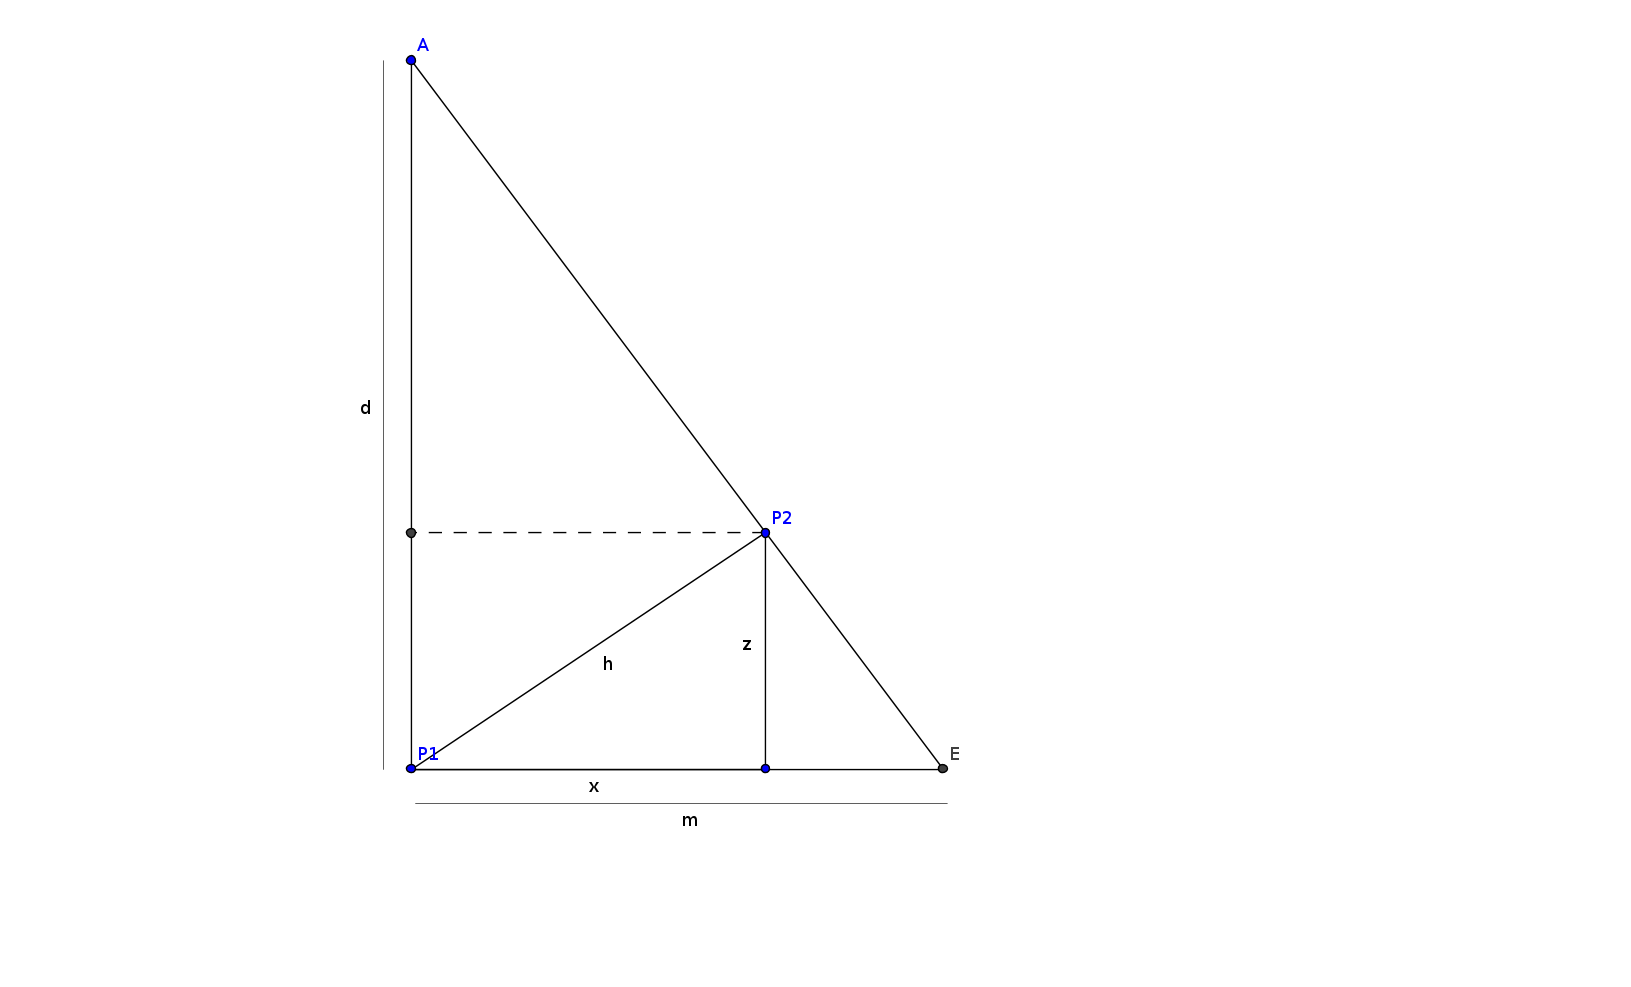
\includegraphics{tales1}
\newpage
Tenemos, usando el teorema de Pitágoras:
\begin{equation*}
h=\sqrt{x^2 + z^2}
\end{equation*}
Y por el Teorema de Tales:
\begin{equation*}
m = \dfrac{h}{d-z}d
\end{equation*}
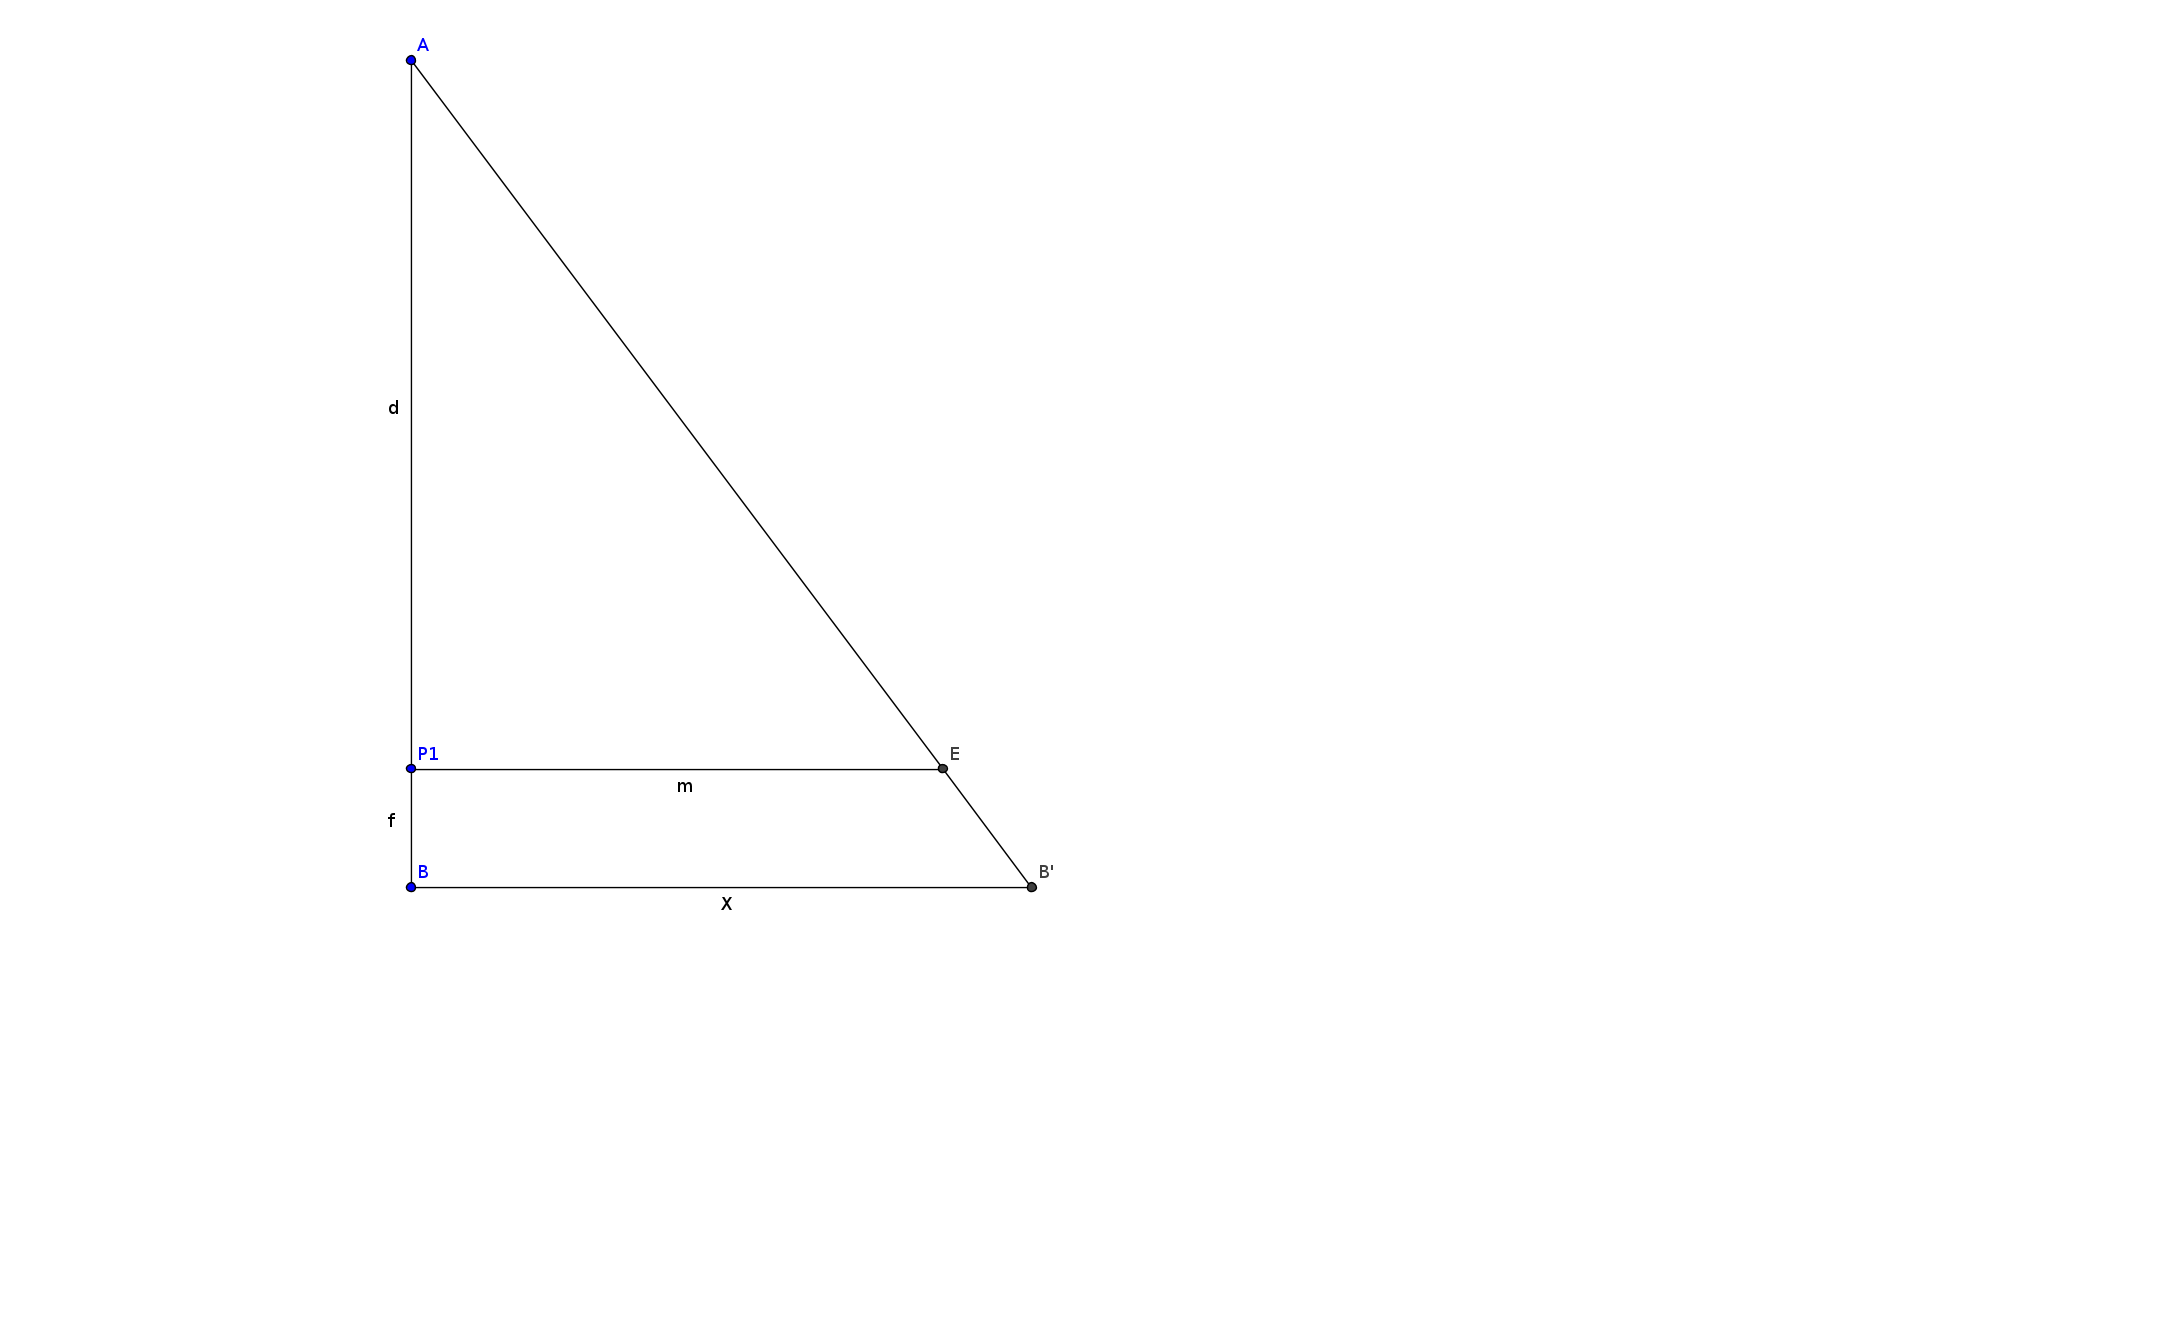
\includegraphics{tales2}
Por último, de nuevo por Tales y por lo anterior, obtenemos que
\begin{equation*}
X=\dfrac{m}{d}(d+f)
\end{equation*}
siendo f la distancia focal de la cámara.
Para obtener el desplazamiento en la imagen en el eje y, los cálculos son análogos.

El código se incluye al final en el apéndice \ref{ap_acc}.
\newpage


\subsection{Resultados}
Lamentablemente este método no produce resultados satisfactorios. En algunas ocasiones, sin llegar a producir buenos resultados, estos parecerían acercarse un poco a lo que desearíamos, otras veces no tanto. Esto es debido  (como apuntan en la charla de Google \textit{Sensor Fusion on Android Devices: A Revolution in Motion Processing} \cite{googlesensor}) principalmente a dos motivos:
\begin{itemize}
\item El primero es por el error producido al aproximar la doble integral que tenemos que calcular para obtener la posición a partir de la aceleración. Según la exposición, manteniendo el dispositivo quieto durante un segundo, se produciría un error de 20 segundos.
\item El segundo motivo es el realmente problemático. Se trata del posible error producido al calcular la aceleración lineal. Recordemos que esto se hacía restando la fuerza de la gravedad de los datos obtenidos por el acelerómetro, y para ello hay que calcular la fuerza de la gravedad. Un pequeño error calculando el ángulo de la gravedad supone un error enorme tras las dos integrales: una diferencia de un grado supondría un error de 8.5 metros.
\end{itemize}

\chapter{Estabilización de la luz}
\section{Introducción}
Por último vamos a ver por encima algunos de los recursos de que disponemos para trabajar con la luz y un algoritmo para intentar estabilizar la iluminación.
\newline
En primer lugar, hablemos de los histogramas. Un histograma es una gráfica que representa frecuencias, en este caso los niveles de intensidad de los píxeles. Es decir, relaciona cada nivel de intensidad de la imagen con el número de píxeles que tienen dicho nivel de intensidad. Por tanto cada canal de la imagen tiene su propio histograma; no obstante nosotros trabajaremos con imágenes en escala de grises, que solo  tienen un único canal.
\newline
Las principales funciones a la hora de trabajar con histogramas son:
\newline
\lstinline|cv2.calcHist(images, channels, mask, histSize, ranges)| y
\newline \lstinline| cv2.equalizeHist(src)|.
La primera se encarga de calcular el histograma y la segunda lo ecualiza.
\newline 
La ecualización de un histograma es un método para mejorar el contraste de la imagen modificando el histograma. La idea intuitiva es encontrar el intervalo del histograma en el que se encuentran la mayor parte de los píxeles y de alguna forma ``alargar'' este intervalo aplanando el histograma. Lo que queremos es transformar una distribución (el histograma original) en otra; para esta transformación usaremos la función de distribución acumulada. Para un histograma $H(i)$, su función de distribución acumulada $H'(i)$ es:
\begin{equation*}
H^{'}(i) = \sum_{0 \le j < i} H(j)
\end{equation*}
Por último tenemos que normalizar para que el valor máximo sea 255:
\begin{equation*}
H^{'}(i) =\frac{H^{'}(i) - \min\{H^{'}(j)\}} {\max\{H^{'}(j)\}-\min\{H^{'}(j)\}} \cdot255
\end{equation*}
Para finalmente poder aplicar la transformación:
\begin{equation*}
equalized( x, y ) = H^{'}( src(x,y) )
\end{equation*}
Otra transformación parecida a la ecualización de un histograma es la normalización. En este caso se ajusta el valor mínimo del histograma al 0 y el máximo al 255, manteniendo la forma original del histograma. Esta operación se puede realizar con la función \lstinline| cv2.normalize()| con los parámetros \lstinline|alpha=0|,\lstinline|beta=255| y \lstinline|norm_type=cv2.NORM_MINMAX|.

\section{Un algoritmo de normalización de luz}
La ecualización es muy importante y es bastante usada para corregir el contraste de la imagen, pero por sí sola es completamente insuficiente a la hora de normalizar la iluminación. En el texto \textit{Enhanced Local Texture Feature Sets for Face Recognition Under Difficult Lighting Conditions} \cite{illuFace} se propone un algoritmo para normalizar la iluminación para la posterior detección de caras.
\newline
Dicho algoritmo consta de tres pasos:
\begin{enumerate}
\item \textbf{Corrección gamma:} 
se trata de una transformación no lineal que dada una imagen $I$ en escala de grises la reemplaza por ${(\frac{I}{255})}^{\gamma}\cdot255$, con $\gamma \in [0,1]$. Utilizaremos como parámetro $\gamma = 0.2$. Para hacer la potencia utilizamos la función \lstinline|cv2.pow(I,| $\gamma$ \lstinline|)|.

\item \textbf{Diferencia gaussiana:} consiste en, dada una imagen, obtener dos imágenes desenfocadas de la original (una más desenfocada que la otra) utilizando filtro gaussiano y luego obtener la diferencia de ambas. Utilizaremos $\sigma_0 =1$ y $\sigma_1=2$ para los filtros y para obtener la diferencia utilizaremos la función \lstinline|cv2.subtract()|

\item \textbf{Ecualización de contraste}: hay que reescalar la intensidad de la imagen para estandarizar el contraste. Un opción podría ser ecualizar o normalizar el histograma, pero en el papel citado proponen un método en dos fases:
\begin{equation}
I(x,y) \leftarrow \frac{I(x,y)}{ {(\text{mean}(|I(x',y')|^a))}^{1/a}}
\end{equation}

\begin{equation}
I(x,y) \leftarrow \frac{I(x,y)}{ {(\text{mean}({\min(\tau, |I(x',y')|)}^a))}^{1/a}}
\end{equation}
Donde $a$ es un componente de compresión y $\tau$ es el umbral de truncamiento. Se usará $a=0.1$ y $\tau=10$.
\end{enumerate}

\section{Corrección de la iluminación usando el sensor}
Nuevamente intentamos usar para nuestros propósitos los sensores de que disponen los telefónos móviles. En este caso intentaremos utilizar los datos que nos proporciona el sensor de luz. Este sensor mide el nivel de luz ambiental en las unidades del Sistema Internacional para la iluminancia o nivel de iluminación, el lux.

La manera de acceder al sensor de luz es análoga a la de acceder al acelerómetro, por lo que los códigos son muy similares y no hay nada diferente de lo ya realizado. En cualquier caso se adjunta el código de la actividad principal en el apéndice \ref{android_ap_illu}.

Una vez que tenemos los lux medidos en cada instante tenemos que ver que podemos hacer con ellos. 

En primer lugar estableceremos una escala, para ello supondremos que nos encontramos en una habitación.En este caso podemos suponer que a partir de 400 lx la habitación está muy iluminada. Por tanto fijamos 400 como el máximo y reescalamos a un  $k \in [0,1]$ dividiendo por 400. Queremos que estos datos representen lo iluminada que está la imagen. 
Como la relación entre lo iluminada que está una imagen y la iluminación ambiental no es lineal, elevamos los datos a un $\alpha  \in [0,1]$, en concreto hemos decidido usar  $\alpha = 1/4$.

Antes de ver cómo usamos estos datos, veamos primero la transformación que proponemos. Se trata de algo que en muchos programas de edición de imagen se conoce como ajuste de niveles. 
La idea es la siguiente, tenemos tres parámetros. Los dos primeros son un límite inferior y un límite superior.  Todos los píxeles de la imagen que tengan una intensidad igual o inferior al límite inferior pasan a ser 0. Análogamente todos los píxeles de la imagen que tengan una intensidad igual o superior pasan a ser 255. El límite inferior y superior pueden tomar valores de 0 a 255 siempre que el inferior sea menor o igual que el superior.
El resto de valores comprendidos entre los límites inferior y superior se transforman al rango [0,255] normalizando y multiplicando por 255.
El último valor(que llamaremos $\gamma$ y supondremos entre 0.1 y 10) lo que hace es desplazar el ``punto medio'' de la imagen, que inicialmente se encuentra en 128 ($\gamma=1$). Esto se realiza con una corrección gamma, elevando las intensidades de cada píxel a $1/\gamma$.

Los datos de que nosotros disponemos parten de la iluminación media y, por tanto podemos relacionarlos con los tonos medios de la imagen. Por tanto lo que queremos es, si la imagen es muy clara oscurecerla disminuyendo $\gamma$ y si es muy oscura, aclararla aumentando $\gamma$.
Esto lo hacemos mediante la transformación $10^{-2k+1}$.
Como límites mínimo y máximo utilizamos los percentiles 1 y 99 respectivamente\footnote{El percentil i-ésimo es aquel valor tal que que un i\% de los valores es menor que él.}.

De las pruebas realizadas podemos observar que el algoritmo funciona bastante bien pero tiene algunas limitaciones: en primer lugar, los cambios bruscos de iluminación,como por otra parte era imaginable,siguen dando problemas, ya que se sigue notando el cambio brusco y, algunas zonas muy oscuras de las imágenes aclaradas siguen quedando totalmente negras. Como ya hemos dicho, esto era esperable. Sin embargo existe otro problema y es que los cambios más leves el sensor algunas veces no los refleja. 
No obstante para cambios no muy bruscos de la iluminación, se puede usar este código, aunque probablemente haya que aplicar posteriormente otro (como el propuesto en el apartado anterior).
Se adjunta el código en el apéndice \ref{ap_illu}.
\appendix
\chapter{Código del acelerómetro} 
\section{Código de Android} \label{android_ap_acc}
A continuación se incluyen las partes más importantes del código de la aplicación de Android.

\subsection{MainActivity}

\lstinputlisting[language=Java, frame= single]{Android/Acelerometro/MainActivity.java}
\newpage

\subsection{Clase vcorderView}
A continuación incluimos el código de la clase \lstinline|vcorderView| que es la clase que se encarga de grabar de la cámara.
\lstinputlisting[language=Java, frame= single]{Android/Acelerometro/vcorderView.java}
\newpage
\subsection{Android manifest}
Ahora vemos el archivo \lstinline|AndroidManifest.xml| en el que cabe destacar las líneas en las que hemos indicado los permisos especiales que necesitamos (el uso de la cámara y de poder escribir en el almacenamiento del móvil).
\lstinputlisting[language=Xml, frame= single]{Android/Acelerometro/AndroidManifest.xml}

\subsection{Activity layout}
Por último vemos el archivo XML que describe la interfaz de nuestra única actividad (y que tan solo es un marco y la zona en la que mostraremos la imagen mientras estemos grabando).
\lstinputlisting[language=Xml, frame= single]{Android/Acelerometro/res/layout/activity_main.xml}

\newpage
\section{Código de procesado de los datos} \label{ap_acc}
A continuación se incluye el programa que procesa los datos recogidos por el programa de Android.
\lstinputlisting[language=Python, frame= single]{estabilizacion_acelerometro.py}
\newpage


\chapter{Código del sensor de luz} 
\section{Código de Android} \label{android_ap_illu}
Solo incluimos el código de la actividad principal, porque el resto de archivos son iguales que los del código del acelerómetro.
\lstinputlisting[language=Java, frame= single]{Android/Luz/MainActivity.java}
\newpage
\section{Código de procesado de los datos} \label{ap_illu}
\lstinputlisting[language=Python, frame= single]{ilum_sensor.py}
\newpage


\cleardoublepage
\addcontentsline{toc}{chapter}{Bibliografía}
\bibliographystyle{plain} % estilo de la bibliografía.
\bibliography{texto} % texto.bib es el fichero donde está salvada la bibliografía.
\nocite{*}


\end{document}
